%%%%%%%%%%%%%%%%%%%%%%%%%%%%%%%%%%%%%%%%%
% baposter Landscape Poster
% LaTeX Template
% Version 1.0 (11/06/13)
%
% baposter Class Created by:
% Brian Amberg (baposter@brian-amberg.de)
%
% This template has been downloaded from:
% http://www.LaTeXTemplates.com
%
% License:
% CC BY-NC-SA 3.0 (http://creativecommons.org/licenses/by-nc-sa/3.0/)
%
%%%%%%%%%%%%%%%%%%%%%%%%%%%%%%%%%%%%%%%%%

%----------------------------------------------------------------------------------------
%	PACKAGES AND OTHER DOCUMENT CONFIGURATIONS
%----------------------------------------------------------------------------------------

\documentclass[landscape,archE,fontscale=0.29]{baposter} % Adjust the font scale/size here

%%% Start of code to add %%%
\usepackage{etoolbox}
\patchcmd\thebibliography
    {\labelsep}
    {\labelsep\itemsep=0pt\relax}
    {}
    {\typeout{Couldn't patch the command}}
%%% End of code to add %%%

\usepackage{url}
\usepackage{lipsum}

\usepackage{graphicx} % Required for including images
\graphicspath{{figures/}} % Directory in which figures are stored

\usepackage{amsmath} % For typesetting math
\usepackage{amssymb} % Adds new symbols to be used in math mode

\usepackage{booktabs} % Top and bottom rules for tables
\usepackage{enumitem} % Used to reduce itemize/enumerate spacing
\usepackage{palatino} % Use the Palatino font
\usepackage[font=small,labelfont=bf]{caption} % Required for specifying captions to tables and figures

\usepackage{multicol} % Required for multiple columns
\setlength{\columnsep}{0.5em} % Slightly increase the space between columns
\setlength{\columnseprule}{0mm} % No horizontal rule between columns

\usepackage{tikz} % Required for flow chart
\usetikzlibrary{shapes,arrows} % Tikz libraries required for the flow chart in the template

\newcommand{\compresslist}{ % Define a command to reduce spacing within itemize/enumerate environments, this is used right after \begin{itemize} or \begin{enumerate}
\setlength{\itemsep}{1pt}
\setlength{\parskip}{0pt}
\setlength{\parsep}{0pt}
}

\definecolor{lightblue}{rgb}{0.145,0.6666,1} % Defines the color used for content box headers

% my macros
\newcommand{\myv}{\vspace{-1mm}}


\begin{document}

\begin{poster}
{
headerborder=closed, % Adds a border around the header of content boxes
colspacing=1em, % Column spacing
bgColorOne=white, % Background color for the gradient on the left side of the poster
bgColorTwo=white, % Background color for the gradient on the right side of the poster
borderColor=lightblue, % Border color
headerColorOne=black, % Background color for the header in the content boxes (left side)
headerColorTwo=lightblue, % Background color for the header in the content boxes (right side)
headerFontColor=white, % Text color for the header text in the content boxes
boxColorOne=white, % Background color of the content boxes
textborder=roundedleft, % Format of the border around content boxes, can be: none, bars, coils, triangles, rectangle, rounded, roundedsmall, roundedright or faded
eyecatcher=true, % Set to false for ignoring the left logo in the title and move the title left
headerheight=0.13\textheight, % Height of the header
headershape=roundedright, % Specify the rounded corner in the content box headers, can be: rectangle, small-rounded, roundedright, roundedleft or rounded
headerfont=\Large\bf\textsc, % Large, bold and sans serif font in the headers of content boxes
%textfont={\setlength{\parindent}{1.5em}}, % Uncomment for paragraph indentation
linewidth=2pt % Width of the border lines around content boxes
}
%----------------------------------------------------------------------------------------
%	TITLE SECTION
%----------------------------------------------------------------------------------------
%
%% {
\includegraphics[height=10em]{img/UniversityOfWaterloo_logo_vert_rgb.png}} % First university/lab logo on the left
{
\includegraphics[height=7.5em]{img/Cheriton_Logo.pdf}} % First university/lab logo on the left
{\bf\textsc{MicroFuge: A Middleware Approach to Providing
    Performance Isolation in Cloud Storage Systems \cite{microfuge14}}\vspace{0.1em}} % Poster title
{\vspace{-2mm}
\textsc{Akshay Singh, \textbf{\underline{Xu Cui}}, Benjamin Cassell, Bernard Wong and
    Khuzaima Daudjee \\ David R. Cheriton School of Computer Science}} % Author names and institution
%% {\includegraphics[height=4em]{logo.png}} % Second university/lab logo on the right

%----------------------------------------------------------------------------------------
%	OBJECTIVES
%----------------------------------------------------------------------------------------

\headerbox{Background}{name=background, column=0, row=0, height=0.70}{
%% Cloud allows sharing which increases resource utilization that in turn reduces costs. However, with increased utilization there is also reduced isolation between tenants. This is especially problematic for cloud storage systems which are highly sensitive to performance interference. Since cloud storage is often the performance bottleneck in cloud application, a lack of performance isolation can lead to unpredictable application latencies.
\textbf{A Cloud Scenario}
\myv
\begin{itemize}
\item Cloud computing allows sharing of resource at the cost of reduced isolation.
\item Storage systems are highly sensitive to performance interference.
\item Lack of perform isolation will lead to unpredictable latencies.
\item In worst case, a particular HTTP request may require 35 database lookups. \cite{facebook2013} %${^{1}}$
\item Amazon reported 100ms of latency cost them 1\% in sales. \cite{linden2006} %${^{2}}$
\item Google found an extra .5 seconds delay caused 20\% drop in search traffic. \cite{linden2006} %${^{2}}$
\end{itemize}

\textbf{Performance Isolation}
\myv
\begin{itemize}
\item One can give clients dedicated resources, however this eliminates cost reduction.
\item \textbf{MicroFuge} aims to meet clients' response time requirement in the shared environment.
\item Represent response time requirements with \textbf{request deadlines}.
\item Provide performance isolation by meeting \textbf{request deadlines}.
\end{itemize}

%% \begin{itemize}\compresslist
%% \item[--] \scriptsize{[1] Nathan Farrington and Alexey Andreyev, Facebook's Data
  %% Center Network Architecture.}
%% \item[--] \scriptsize{[2] Greg Lindem, Make Data Useful,
  %% \url{http://www.scribd.com/doc/4970486/Make-Data-Useful-by-Greg-Linden-Amazon-com}.}
%% \end{itemize}
\vspace{0.2em} % When there are two boxes, some whitespace may need to be added if the one on the right has more content
}


\headerbox{MicroFuge}{name=microfuge,column=1,span=2,row=0, height=0.33}{
\begin{multicols*}{2}
\vspace{1em}
A distributed caching and scheduling middleware that provides performance isolation.

\vspace{.5em}
\textbf{Deadline Cache (DLC)}
\myv
\myv
\begin{itemize}\compresslist
\item Builds a performance model.
\item Uses multiple LRU queues for deadline-ware evictions
\end{itemize}

\textbf{Deadline Scheduler (DLS)}
\myv
\myv
\begin{itemize}\compresslist
\item Performs intelligent replica selection.
\item Implements feedback-driven deadline-aware scheduling.
\item Optionally performs admission control.
\end{itemize}
\vspace{3 mm}
\begin{center}
  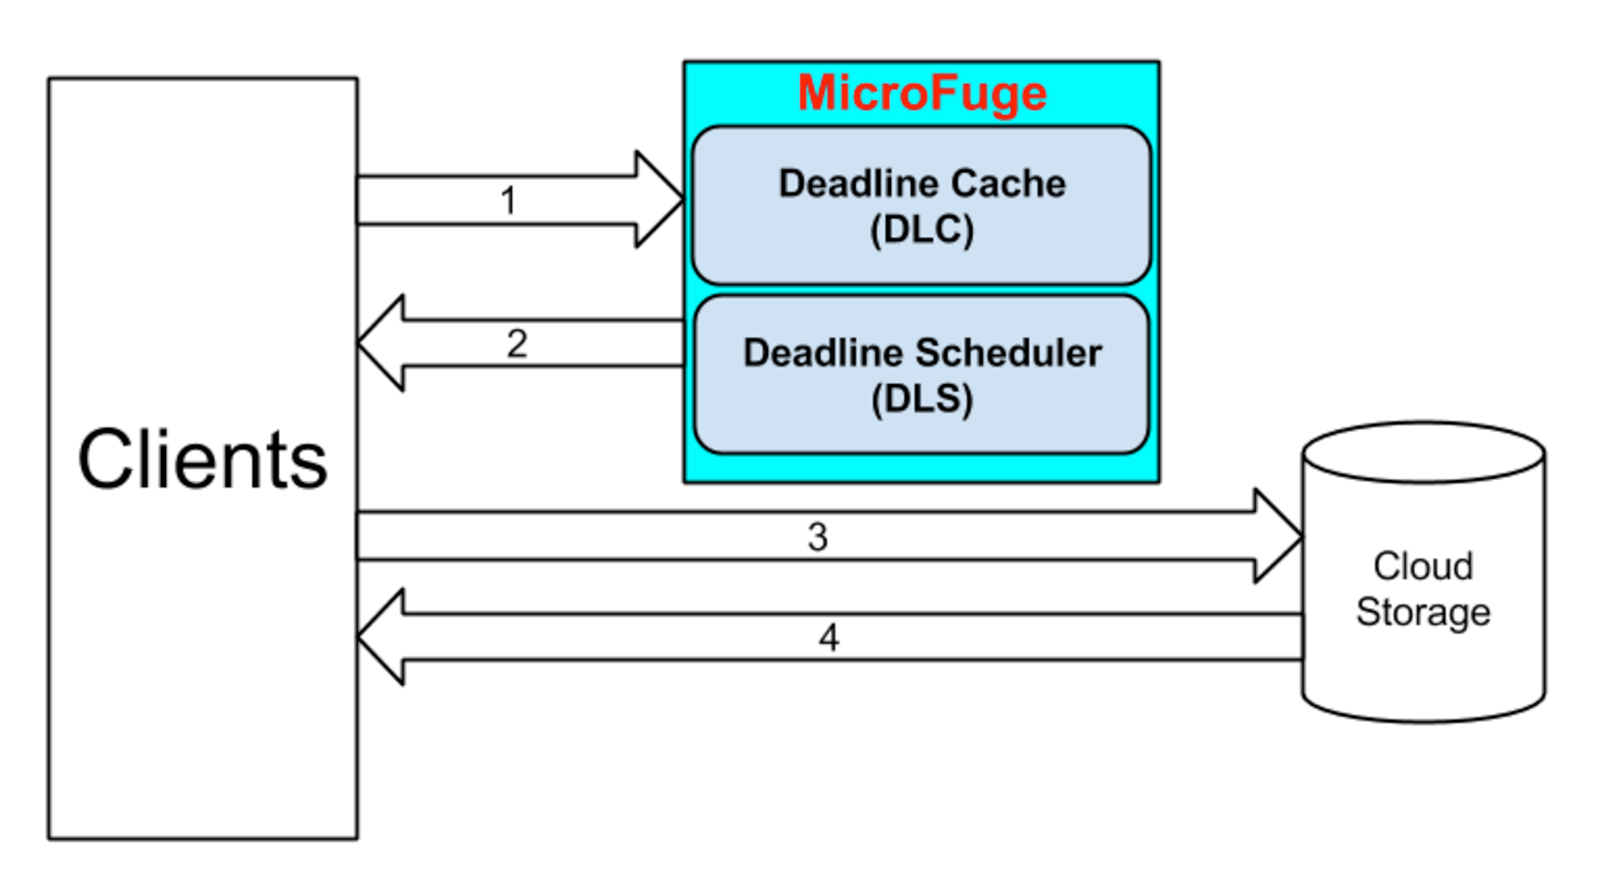
\includegraphics[scale=0.290]{img/MF_FULL_V8_4.pdf}
  \captionof{figure}{System Overview}
\end{center}
\end{multicols*}
\vspace{0.2em} % When there are two boxes, some whitespace may need to be added if the one on the right has more content
}


\headerbox{Deadline Cache}{name=cache, column=1, span=2, below=microfuge, bottomaligned=background}{
  \textbf{DLC} offers adaptive deadline-aware caching.
  \myv \myv \myv
\begin{multicols}{2}
  \begin{itemize}\compresslist
  \item Multiple LRU queues enable DLC to perform deadline-aware evictions.
  \item Each eviction victim is selected by computing the \textit{Modified Recency Value}
    \begin{equation}
      {Current\_Timestamp - Stored\_Timestamp \over Queue\_Specific\_Divisor}
    \end{equation}
  \item \textbf{DLC} uses an adaptive policy that considers both the client request rate for each deadline range and the underlying system's performance to update the adaptive divisors.
  \end{itemize}
  \begin{center}
    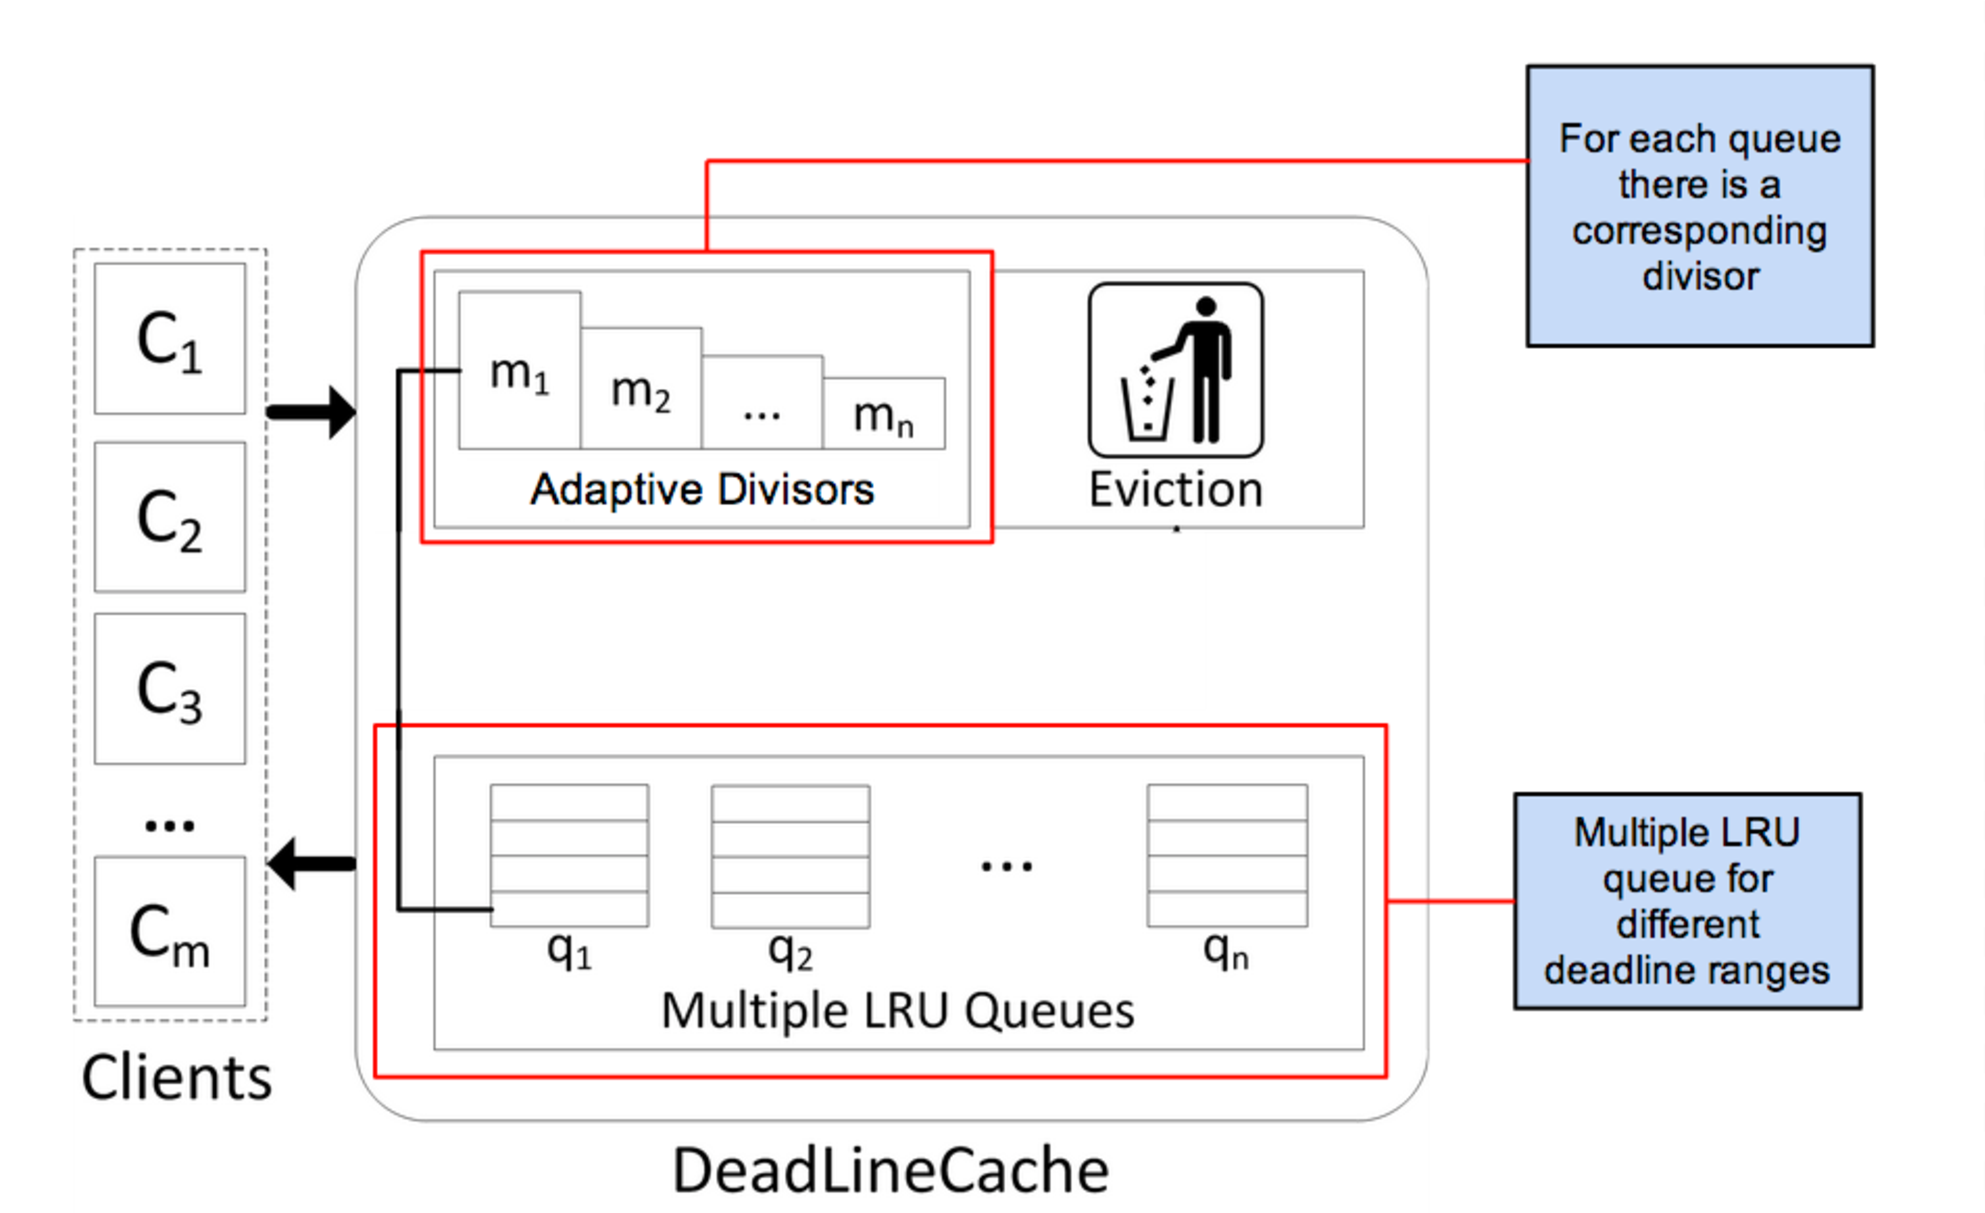
\includegraphics[scale=0.22]{img/DLC_ARC_2.pdf}
    \captionof{figure}{Deadline Cache}
  \end{center}
\end{multicols}
}

\headerbox{Deadline Scheduler}{name=scheduler, column=3, span=1,  bottomaligned=background}{
  With \textbf{MicroFuge}'s distributed design, each \textbf{DLS} is responsible for  scheduling client access to a subset of distributed data servers.
  Each scheduler performs three tasks to provide performance isolation in the scheduling layer.
  \begin{itemize}
  \item \textbf{DLS} will select the replica which is most likely to meet request's deadline.
  \item In order to make the selection, \textbf{DLS} relies on the latency modeling component which uses previous request latencies to predict incoming request's latency.
  \item There are cases where server load just exceeds its capacity. \textbf{DLS} additionally provides an optional admission control mechanism which performs early rejection of requests which are likely to miss their deadlines.
  \end{itemize}
  \myv \myv \myv \myv \myv \myv \myv \myv
  \begin{center}
    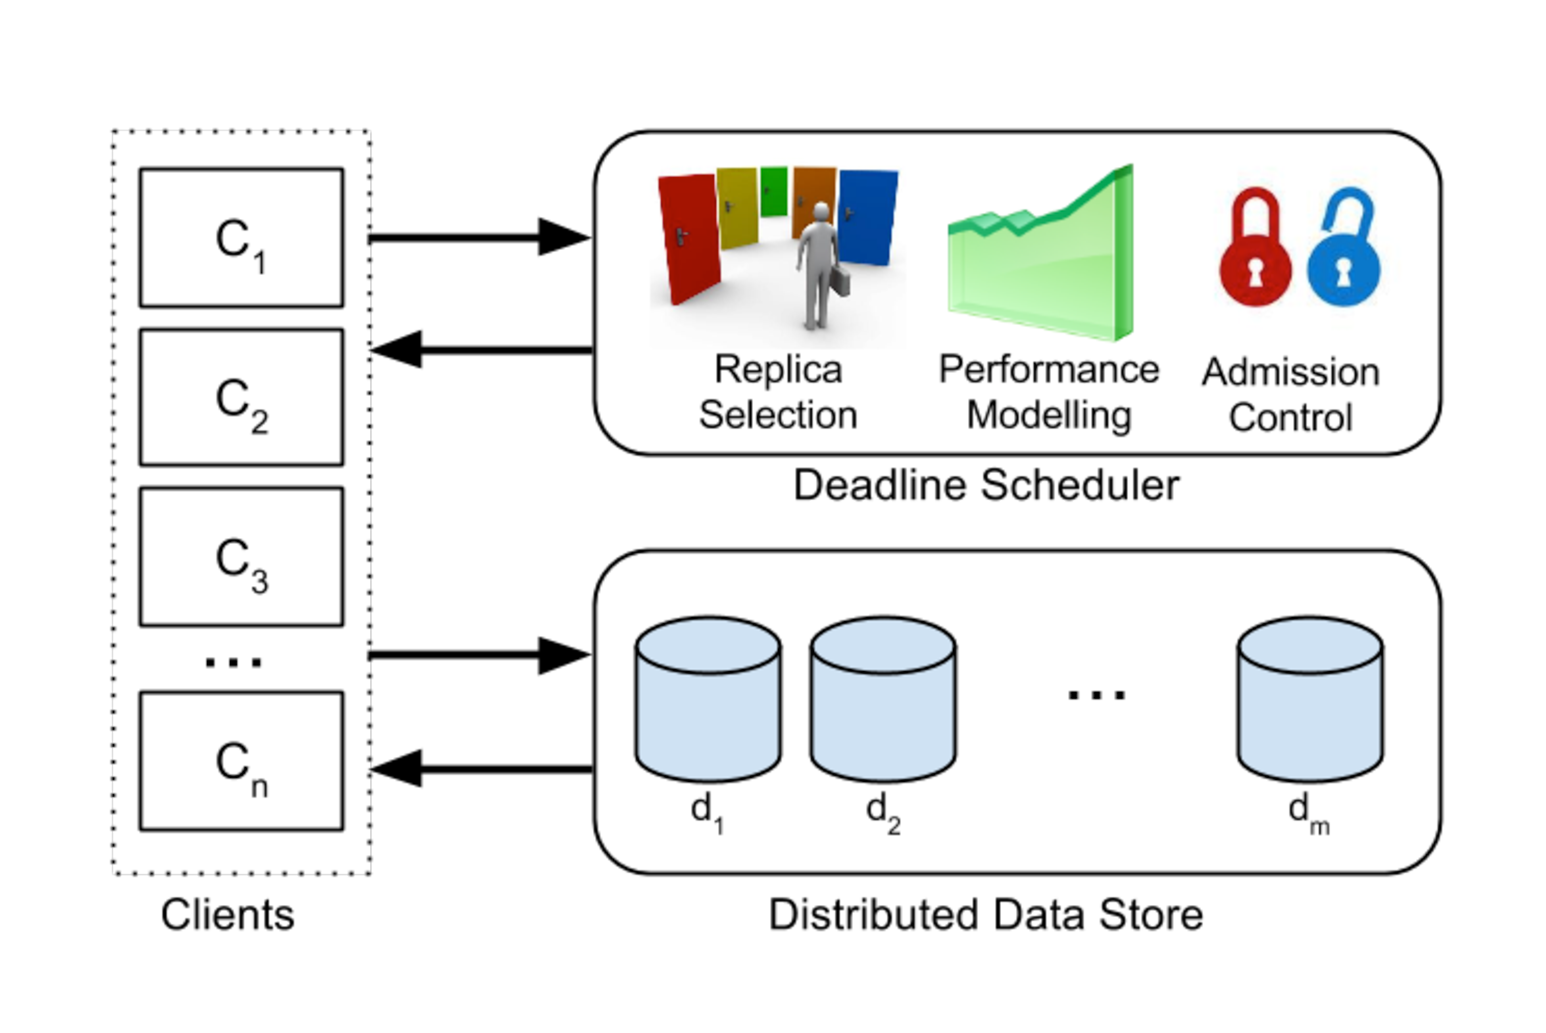
\includegraphics[scale=0.25]{img/DLS_ARCH_4.pdf}
    \captionof{figure}{Deadline Scheduler}
  \end{center}
}

\headerbox{References}{name=reference, column=0,below=background, above=bottom}{
  \renewcommand{\section}[2]{\vskip 0.05em%
  } % Get rid of the default ``References'' section title

  \nocite{*} % Insert publications even if they are not cited in the poster
  \small{ % Reduce the font size in this block
    \bibliographystyle{unsrt}
    \bibliography{microfuge} % Use sample.bib as the bibliography file
  }
  %% [1] A. Singh, X. Cui, B. Cassell, B. Wong, K. Daudjee, MicroFuge: A Middleware Approach to Providing Performance Isolation in Cloud Storage Systems, in 34th IEEE International Conference on Distributed Computing Systems (ICDCS).

  %% [2] Nathan Farrington and Alexey Andreyev, Facebook's Data
  %% Center Network Architecture.

  %% [3] Greg Lindem, Make Data Useful,
  %% \footnotesize{\url{http://www.scribd.com/doc/4970486/Make-Data-Useful-by-Greg-Linden-Amazon-com}.}
}

\headerbox{Performance Evaluation}{name=performance, column=1, span=2,below=background, above=bottom}{
  \begin{multicols}{3}

    \begin{flushleft}
      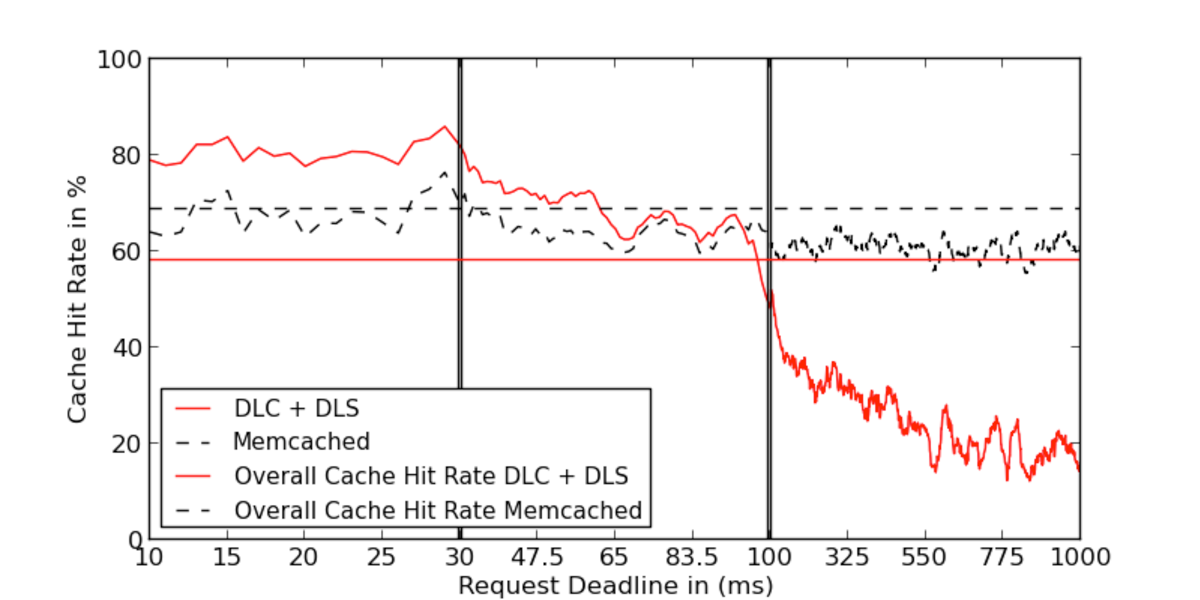
\includegraphics[scale=0.27]{img/EC2/EC2_SH_MM/cache_48.pdf}
      \captionof{figure}{Cache Hit Rate}
    \end{flushleft}
    \vspace{0.5em}
    \begin{flushleft}
      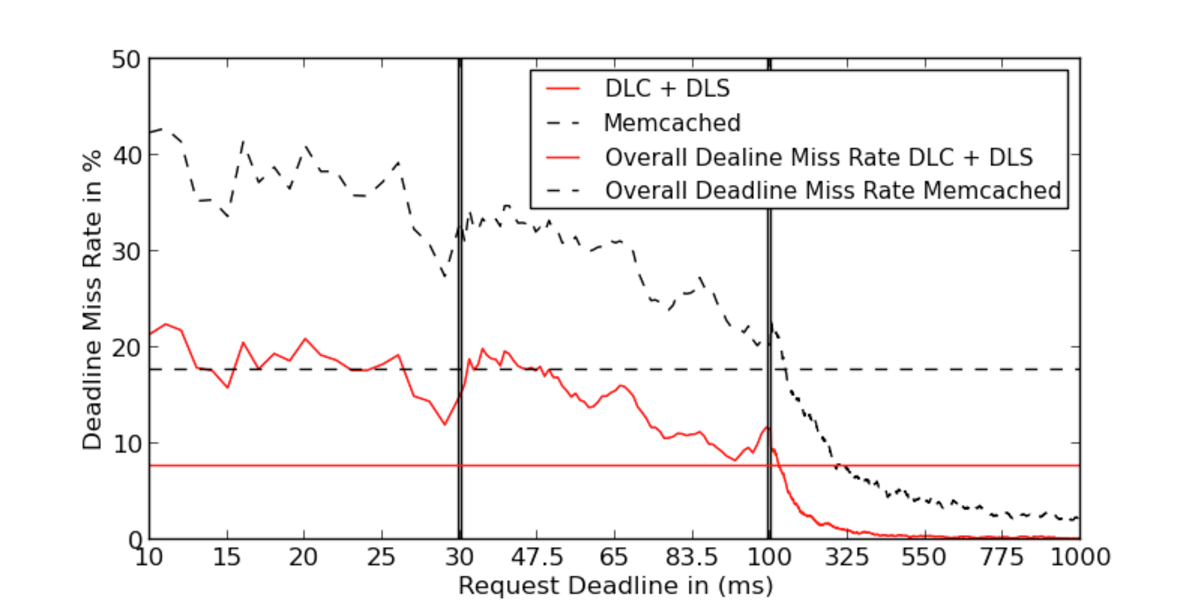
\includegraphics[scale=0.27]{img/EC2/EC2_SH_MM/miss_48.pdf}
      \captionof{figure}{Deadline Miss Rate}
    \end{flushleft}
    \vspace{0.5em}
    \center\textbf{Experimental Setup}
    \myv
    \begin{itemize}\compresslist
      \vspace{-1.57mm}
    \item Twenty-node test cluster on AWS. Each cluster node is an m1.medium EC2 instance.
    \item Benchmarking System: Yahoo! Cloud Serving
      Benchmark (YCSB). Modified to assign different ranges of deadlines to each key.
    \end{itemize}
  \end{multicols}
}
\headerbox{Conclusion}{name=conclusion, column=3,below=background, above=bottom}{
  \vspace{1em}
  \begin{itemize}
  \item Predictable performance is necessary in multi-tenant environments.
  \item MicroFuge tackles the performance isolation problem with its deadline-aware caching and scheduling middleware.
  \item MicroFuge reduces deadline miss rate from 17.5\% to 7.7\% and it can be as low as 4.7\% if we turn on the admission control.
  \end{itemize}
}
\end{poster}

\end{document}
